\section{Trigger Class Reference}
\label{classTrigger}\index{Trigger@{Trigger}}
Abstract class for all triggers.  


{\tt \#include $<$trigger.hpp$>$}

Inheritance diagram for Trigger::\begin{figure}[H]
\begin{center}
\leavevmode
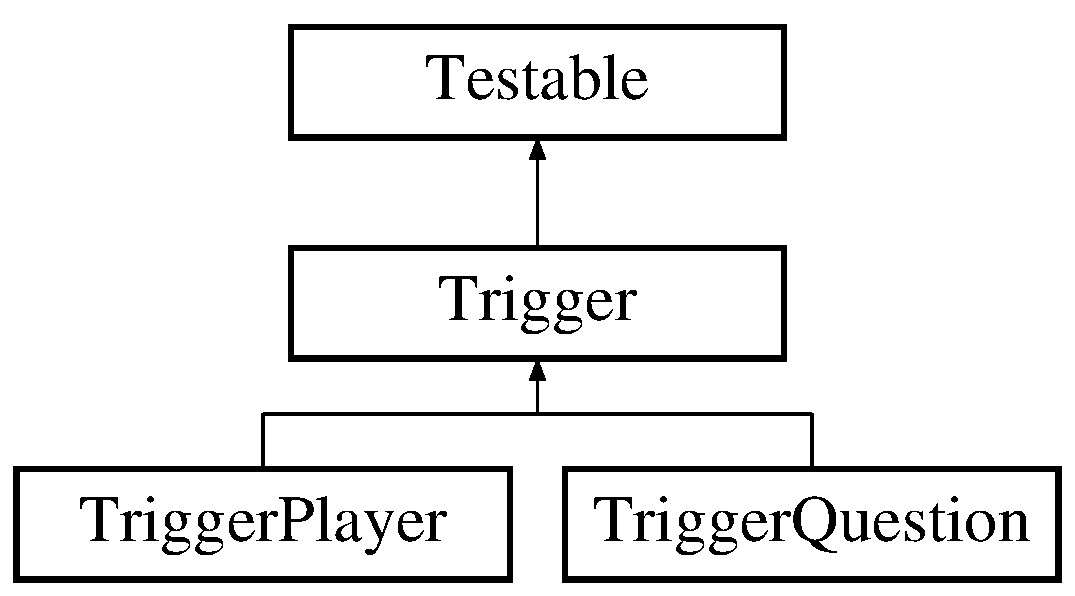
\includegraphics[height=3cm]{classTrigger}
\end{center}
\end{figure}
\subsection*{Public Member Functions}
\begin{CompactItemize}
\item 
{\bf Trigger} ()
\item 
virtual {\bf $\sim$Trigger} ()
\item 
void {\bf load} ({\bf Parser} \&parser)
\item 
void {\bf save} (ofstream \&file) const 
\item 
bool {\bf activate} ({\bf Monster} \&monster)
\item 
virtual bool {\bf can\-Activate} ({\bf Monster} \&monster)=0
\item 
QList$<$ {\bf QInts\-Pair} $>$ {\bf get\-Points} () const 
\item 
virtual QString {\bf name} () const =0
\item 
int {\bf test} (bool verbose) const 
\end{CompactItemize}
\subsection*{Protected Member Functions}
\begin{CompactItemize}
\item 
virtual void {\bf cust\-Load} ({\bf Parser} \&parser)=0
\item 
virtual void {\bf cust\-Save} (ofstream \&file) const =0
\item 
void {\bf save\-Actions} (ofstream \&file) const 
\item 
void {\bf load\-Actions} ({\bf Parser} \&parser)
\end{CompactItemize}
\subsection*{Protected Attributes}
\begin{CompactItemize}
\item 
QList$<$ {\bf Abstract\-Action} $\ast$ $>$ {\bf actions}
\item 
{\bf Coordinates\-List} {\bf coordinates}
\item 
int {\bf duration}
\end{CompactItemize}


\subsection{Detailed Description}
Abstract class for all triggers. 



\subsection{Constructor \& Destructor Documentation}
\index{Trigger@{Trigger}!Trigger@{Trigger}}
\index{Trigger@{Trigger}!Trigger@{Trigger}}
\subsubsection{\setlength{\rightskip}{0pt plus 5cm}{\bf Trigger} ()}\label{classTrigger_a0}


\index{Trigger@{Trigger}!~Trigger@{$\sim$Trigger}}
\index{~Trigger@{$\sim$Trigger}!Trigger@{Trigger}}
\subsubsection{\setlength{\rightskip}{0pt plus 5cm}$\sim${\bf Trigger} ()\hspace{0.3cm}{\tt  [virtual]}}\label{classTrigger_a1}




\subsection{Member Function Documentation}
\index{Trigger@{Trigger}!activate@{activate}}
\index{activate@{activate}!Trigger@{Trigger}}
\subsubsection{\setlength{\rightskip}{0pt plus 5cm}bool activate ({\bf Monster} \& {\em monster})}\label{classTrigger_a4}


\index{Trigger@{Trigger}!canActivate@{canActivate}}
\index{canActivate@{canActivate}!Trigger@{Trigger}}
\subsubsection{\setlength{\rightskip}{0pt plus 5cm}virtual bool can\-Activate ({\bf Monster} \& {\em monster})\hspace{0.3cm}{\tt  [pure virtual]}}\label{classTrigger_a5}




Implemented in {\bf Trigger\-Player} {\rm (p.\,\pageref{classTriggerPlayer_a2})}, and {\bf Trigger\-Question} {\rm (p.\,\pageref{classTriggerQuestion_a4})}.\index{Trigger@{Trigger}!custLoad@{custLoad}}
\index{custLoad@{custLoad}!Trigger@{Trigger}}
\subsubsection{\setlength{\rightskip}{0pt plus 5cm}virtual void cust\-Load ({\bf Parser} \& {\em parser})\hspace{0.3cm}{\tt  [protected, pure virtual]}}\label{classTrigger_b0}




Implemented in {\bf Trigger\-Player} {\rm (p.\,\pageref{classTriggerPlayer_b0})}, and {\bf Trigger\-Question} {\rm (p.\,\pageref{classTriggerQuestion_a2})}.\index{Trigger@{Trigger}!custSave@{custSave}}
\index{custSave@{custSave}!Trigger@{Trigger}}
\subsubsection{\setlength{\rightskip}{0pt plus 5cm}virtual void cust\-Save (ofstream \& {\em file}) const\hspace{0.3cm}{\tt  [protected, pure virtual]}}\label{classTrigger_b1}




Implemented in {\bf Trigger\-Player} {\rm (p.\,\pageref{classTriggerPlayer_b1})}, and {\bf Trigger\-Question} {\rm (p.\,\pageref{classTriggerQuestion_a3})}.\index{Trigger@{Trigger}!getPoints@{getPoints}}
\index{getPoints@{getPoints}!Trigger@{Trigger}}
\subsubsection{\setlength{\rightskip}{0pt plus 5cm}QList$<$ {\bf QInts\-Pair} $>$ get\-Points () const}\label{classTrigger_a6}


\index{Trigger@{Trigger}!load@{load}}
\index{load@{load}!Trigger@{Trigger}}
\subsubsection{\setlength{\rightskip}{0pt plus 5cm}void load ({\bf Parser} \& {\em parser})}\label{classTrigger_a2}


\index{Trigger@{Trigger}!loadActions@{loadActions}}
\index{loadActions@{loadActions}!Trigger@{Trigger}}
\subsubsection{\setlength{\rightskip}{0pt plus 5cm}void load\-Actions ({\bf Parser} \& {\em parser})\hspace{0.3cm}{\tt  [protected]}}\label{classTrigger_b3}


\index{Trigger@{Trigger}!name@{name}}
\index{name@{name}!Trigger@{Trigger}}
\subsubsection{\setlength{\rightskip}{0pt plus 5cm}virtual QString name () const\hspace{0.3cm}{\tt  [pure virtual]}}\label{classTrigger_a7}




Implemented in {\bf Trigger\-Player} {\rm (p.\,\pageref{classTriggerPlayer_a3})}, and {\bf Trigger\-Question} {\rm (p.\,\pageref{classTriggerQuestion_a5})}.\index{Trigger@{Trigger}!save@{save}}
\index{save@{save}!Trigger@{Trigger}}
\subsubsection{\setlength{\rightskip}{0pt plus 5cm}void save (ofstream \& {\em file}) const}\label{classTrigger_a3}


\index{Trigger@{Trigger}!saveActions@{saveActions}}
\index{saveActions@{saveActions}!Trigger@{Trigger}}
\subsubsection{\setlength{\rightskip}{0pt plus 5cm}void save\-Actions (ofstream \& {\em file}) const\hspace{0.3cm}{\tt  [protected]}}\label{classTrigger_b2}


\index{Trigger@{Trigger}!test@{test}}
\index{test@{test}!Trigger@{Trigger}}
\subsubsection{\setlength{\rightskip}{0pt plus 5cm}int test (bool {\em verbose}) const\hspace{0.3cm}{\tt  [virtual]}}\label{classTrigger_a8}




Implements {\bf Testable} {\rm (p.\,\pageref{classTestable_a0})}.

\subsection{Member Data Documentation}
\index{Trigger@{Trigger}!actions@{actions}}
\index{actions@{actions}!Trigger@{Trigger}}
\subsubsection{\setlength{\rightskip}{0pt plus 5cm}QList$<${\bf Abstract\-Action}$\ast$$>$ {\bf actions}\hspace{0.3cm}{\tt  [protected]}}\label{classTrigger_p0}


\index{Trigger@{Trigger}!coordinates@{coordinates}}
\index{coordinates@{coordinates}!Trigger@{Trigger}}
\subsubsection{\setlength{\rightskip}{0pt plus 5cm}{\bf Coordinates\-List} {\bf coordinates}\hspace{0.3cm}{\tt  [protected]}}\label{classTrigger_p1}


\index{Trigger@{Trigger}!duration@{duration}}
\index{duration@{duration}!Trigger@{Trigger}}
\subsubsection{\setlength{\rightskip}{0pt plus 5cm}int {\bf duration}\hspace{0.3cm}{\tt  [protected]}}\label{classTrigger_p2}




The documentation for this class was generated from the following files:\begin{CompactItemize}
\item 
{\bf trigger.hpp}\item 
{\bf trigger.cpp}\end{CompactItemize}
